% =============================================================================
% CSE 445: Machine Learning -- Project Report, Summer 2026
%
% Structure follows "CSE445_Project_Report_Guideline_Summer_2026" (sections
% 1-12 + references) and the cover page / individual-contribution table of
% "CSE 445_Project_Final_Report_IEEE_Format_Summer_2026.docx".
% Typeset in IEEE conference format as the guideline requires.
%
% Build: pdflatex report.tex   (run twice)
%
% ---------------------------------------------------------------------------
% ITEMS THAT MUST BE FILLED IN BEFORE SUBMISSION are wrapped in \FILL{...}
% and printed in red so they cannot be missed. Search for "FILL".
% ---------------------------------------------------------------------------
\documentclass[conference]{IEEEtran}
\IEEEoverridecommandlockouts

\usepackage{cite}
\usepackage{amsmath,amssymb,amsfonts}
\usepackage{graphicx}
\usepackage{textcomp}
\usepackage{xcolor}
\usepackage{booktabs}
\usepackage{multirow}
\usepackage{array}
\usepackage{tabularx}
\usepackage{url}
\usepackage[hidelinks]{hyperref}

\newcommand{\FILL}[1]{\textcolor{red}{\textbf{[#1]}}}
\newcommand{\Loss}{\mathcal{L}}


\setcounter{topnumber}{2}
\setcounter{totalnumber}{4}
\renewcommand{\topfraction}{0.92}
\renewcommand{\textfraction}{0.06}
\renewcommand{\floatpagefraction}{0.65}

\title{DASF-Net: Dual-Adversarial Spectral Fusion for\\
Cross-Lingual and Adversarially Robust Audio Deepfake Detection}

\author{
\IEEEauthorblockN{Iftikhar Ahmed,\quad Meherun Nessa Mithila}
\IEEEauthorblockA{\textit{Department of Electrical and Computer Engineering}\\
\textit{North South University}, Dhaka, Bangladesh\\
\{iftikhar.ahmed,\ meherun.mithila\}@northsouth.edu}
}

\begin{document}

% =============================================================================
% COVER PAGE + INDIVIDUAL CONTRIBUTION TABLE  (guideline section 1)
% The titlepage environment switches to one column and restores two columns.
% =============================================================================
\begin{titlepage}
\centering
\vspace*{1.2cm}

{\large Department of Electrical and Computer Engineering}\\[4pt]
{\large North South University}\\[28pt]

{\LARGE\bfseries CSE 445 Report}\\[36pt]

\rule{0.85\textwidth}{0.6pt}\\[14pt]
{\LARGE\bfseries DASF-Net: Dual-Adversarial Spectral Fusion for
Cross-Lingual and Adversarially Robust Audio Deepfake Detection}\\[14pt]
\rule{0.85\textwidth}{0.6pt}\\[40pt]

\begin{tabular}{@{}l@{\hspace{2.5cm}}l@{}}
\textbf{Name} & \textbf{ID} \\[4pt]
Iftikhar Ahmed         & 2121019642 \\[4pt]
Meherun Nessa Mithila  & 2221649042 \\[4pt]
\end{tabular}

\vspace{40pt}

\textbf{Faculty:}\\[6pt]
Mohammad Abdul Qayum (MAQM)\\
Assistant Professor\\
ECE Department\\[30pt]

\textbf{Course / Section:}\ CSE 445, Section 6\\[6pt]
\textbf{Date of Submission:}\ 6 September 2026\\[24pt]

{\large\bfseries Summer 2026}

\vfill

\newpage

% ---------------------------------------------------------------------------
\centering
{\large\bfseries Individual Contribution Table}\\[16pt]

\begin{tabularx}{0.92\textwidth}{@{}>{\raggedright\arraybackslash}X
                                   >{\raggedright\arraybackslash}X@{}}
\toprule
\textbf{Section} & \textbf{Contributing Member} \\
\midrule
IEEE / \LaTeX{} formatting                    & Iftikhar Ahmed \\
Grammarly check                               & Meherun Nessa Mithila \\
Grammarly score                               & 58 \\
Abstract                                      & Iftikhar Ahmed \\
Keywords                                      & Meherun Nessa Mithila \\
Introduction, motivation                      & Meherun Nessa Mithila \\
Paper review 1 --- BanglaFake                 & Meherun Nessa Mithila \\
Paper review 2 --- Mel-Spectrogram / Xception & Iftikhar Ahmed \\
Paper review 3 --- Zero-Shot to Zero-Lies     & Meherun Nessa Mithila \\
Paper review 4 --- WaveFake                   & Iftikhar Ahmed \\
Paper review 5 --- Kawa \emph{et al.}, adversarial defence & Meherun Nessa Mithila \\
Introduction, description of our own work     & Iftikhar Ahmed \\
Proposed system (dataset and preprocessing)   & Meherun Nessa Mithila \\
Proposed system (model description)           & Iftikhar Ahmed \\
Testing methodology and evaluation protocol   & Iftikhar Ahmed \\
Timeline and budget                           & Meherun Nessa Mithila \\
Risk analysis and mitigation                  & Iftikhar Ahmed \\
Figure and table title formatting             & Meherun Nessa Mithila \\
Equations formatting                          & Iftikhar Ahmed \\
Conclusions                                   & Iftikhar Ahmed \\
References formatting in IEEE format          & Meherun Nessa Mithila \\
\bottomrule
\end{tabularx}

\vspace{10pt}
{\small Ten sections each; the two members contributed equally to this report.}

\vfill
\end{titlepage}

% =============================================================================
\maketitle

% ----------------------------------------------------- guideline 2: abstract
\begin{abstract}
Audio deepfake detectors are trained and evaluated almost exclusively on
high-resource languages and on a narrow family of neural vocoders. When such a
detector meets a new language synthesised by a structurally different
generator, two failure modes compound: the learned features encode language-
and corpus-specific cues rather than synthesis artifacts, and the decision
boundary remains trivially breakable by gradient-based perturbation. This
project proposes \textbf{DASF-Net}, a detection architecture built on the
observation that these two failures are both \emph{adversarial} problems and
can be addressed by a single training formulation. DASF-Net couples (i) a
dual-branch spectral front-end that presents the same utterance as a sparse
cepstral view (LFCC) and a dense spectral view (log-Mel) to one
Siamese-shared, ImageNet-pretrained Xception trunk; (ii) a Cross-Attention
Spectral Fusion (CASF) module that lets the two views query one another and
combines them through a learned gate, so that the network selects per
utterance which representation carries the artifact; and (iii) a
dual-adversarial objective in which a gradient-reversed language discriminator
drives the embedding toward language invariance while adaptive FGSM/PGD
adversarial training drives it toward perturbation robustness. A three-stage
curriculum trains these parts in a stable order. The design is instantiated on
the English WaveFake corpus (117,985 utterances, seven GAN- and flow-based
vocoders) as source domain and the Bengali BanglaFake corpus (25,520
utterances, one VITS end-to-end system) as target domain, a pairing that
varies language and synthesis paradigm simultaneously. A Confound-Controlled
Evaluation Protocol is specified to neutralise the speaker, gender and
class-prior imbalances that otherwise inflate Bengali detection scores. The
expected impact is the first cross-lingual, adversarially evaluated benchmark
for Bengali audio deepfake detection, together with a reusable methodology for
extending it to other low-resource languages. \textbf{This report covers the
design, architecture, algorithms and experimental plan; the experiments have
not yet been executed and no results are reported.}
\end{abstract}

\begin{IEEEkeywords}
machine learning, audio deepfake detection, cross-lingual generalisation,
adversarial robustness, domain-adversarial training, cross-attention fusion,
Mel-spectrogram, Xception, convolutional neural networks, Bengali speech,
low-resource language, equal error rate
\end{IEEEkeywords}

% =============================================================================
\section{Introduction, Objectives, Motivation and Contributions}
% ------------------------------------------------- guideline 3
Neural vocoders and end-to-end text-to-speech (TTS) systems now produce speech
that listeners routinely fail to separate from genuine recordings
\cite{kong2020hifigan,kumar2019melgan,prenger2019waveglow,yamamoto2020pwg,kim2021vits}.
The resulting misuse --- voice-impersonation fraud, fabricated evidence,
political disinformation --- has driven a large body of work on automatic
detection \cite{todisco2019asvspoof,frank2021wavefake}. That work is
overwhelmingly English and is overwhelmingly built on a single family of
generators.

Bengali, with more than 230 million native speakers, has almost no detection
literature. BanglaFake \cite{fahad2025banglafake} first made Bengali deepfake
audio available at scale but trained no detector, and ``Zero-Shot to
Zero-Lies'' \cite{samu2025zeroshot} first benchmarked detectors on it,
reporting a best zero-shot result of 53.80\% accuracy (46.20\% EER,
Wav2Vec2-XLSR-53) and a best fine-tuned result of 79.17\% accuracy (24.35\%
EER, ResNet18). Those numbers expose a gap that is not merely quantitative. A
detector that transfers this poorly is not simply under-trained; it has
learned the wrong thing --- its features encode which corpus, which speaker
and which language produced an utterance, rather than what a synthesiser did
to it.

\subsection{Motivation}
The same detectors are, as a large body of adversarial work shows, breakable
by perturbations far below the audible threshold. Kawa \emph{et al.}
\cite{kawa2023lcnn} degrade an LCNN countermeasure from 0.022 to 0.785 EER
under FGSM, and our group's prior study \cite{ahmed2026melspec} reproduces the
pattern on a much larger ImageNet-pretrained Xception detector.

Our position is that these two failures share a structure. In both cases the
network has latched onto a \emph{nuisance direction} in feature space ---
language and corpus identity in one case, a locally exploitable gradient
direction in the other. In both cases the standard remedy is to introduce an
adversary that penalises exactly that direction. Domain-adversarial training
\cite{ganin2016dann} supplies the first adversary; FGSM/PGD adversarial
training \cite{goodfellow2015fgsm,madry2018pgd} supplies the second. Placing
both on a single shared embedding is, to our knowledge, new for audio deepfake
detection, and it turns the cross-lingual question from a measurement exercise
into an architectural one.

\subsection{Objectives}
The project pursues four measurable objectives.

\begin{itemize}
\item \textbf{Objective 1.} Design and implement DASF-Net, a dual-branch
      detector that fuses LFCC and log-Mel views through learned
      cross-attention over a weight-shared Xception trunk, and verify that the
      implementation is correct by shape and gradient tests.
\item \textbf{Objective 2.} Establish an in-language Bengali baseline and
      determine whether the dense-over-sparse representation advantage
      reported for English CNN detectors \cite{ahmed2026melspec} replicates on
      Bengali VITS audio, measured by Equal Error Rate (EER) against the
      published ResNet18 baseline of 0.2435 EER \cite{samu2025zeroshot}.
\item \textbf{Objective 3.} Quantify zero-shot English$\leftrightarrow$Bengali
      transfer with and without the language adversary, and report the
      reduction in EER attributable to domain-adversarial alignment.
\item \textbf{Objective 4.} Measure whether adversarial robustness acquired in
      one language survives transfer to the other, reporting clean, FGSM and
      PGD EER on a single, unit-consistent $\epsilon$ grid.
\end{itemize}

\subsection{Contributions}
\begin{enumerate}
\item \textbf{DASF-Net}, an architecture that presents sparse cepstral and
      dense spectral views of one utterance to a single Siamese-shared
      Xception trunk and fuses them with a two-way cross-attention module and
      a learned gate.
\item A \textbf{dual-adversarial objective} combining a gradient-reversed
      language discriminator with adaptive FGSM/PGD adversarial training on
      the same fused embedding, plus a three-stage curriculum that makes the
      combination trainable.
\item A \textbf{Confound-Controlled Evaluation Protocol} (CCEP) for
      Bengali--English deepfake transfer, which neutralises the speaker,
      gender and class-prior artifacts that make naive BanglaFake accuracy
      figures uninterpretable.
\item A \textbf{corrected, unit-consistent adversarial threat model} that
      places FGSM and PGD on one shared $\epsilon$ grid, resolving an
      inconsistency present in our group's own earlier work.
\item An \textbf{ablation-first experimental design}, so that any
      cross-lingual gain can be attributed to a specific component rather
      than merely observed.
\end{enumerate}

% =============================================================================
\section{Project Background}
% ------------------------------------------------- guideline 4

\subsection{Context and Rationale}
Speech synthesis has moved in a decade from concatenative systems with audible
seams to neural systems whose output is, for untrained listeners, transparent.
The BanglaFake authors report a Mean Opinion Score of 3.40 for naturalness and
4.01 for intelligibility on their Bengali synthetic speech
\cite{fahad2025banglafake}, and their t-SNE visualisation of MFCC features
shows the real and synthetic clusters overlapping heavily. In other words, the
material is already good enough to deceive, and simple cepstral features are
already insufficient to separate it.

The rationale for this project is that detection research has not kept pace in
two specific directions. First, detectors are validated within one language,
so nothing is known about their behaviour when deployed in another. Second,
detectors are validated against passive forgeries rather than an active
adversary who can compute gradients. A deployed countermeasure faces both
conditions simultaneously.

\subsection{Historical and Scientific Context}
Anti-spoofing countermeasures grew out of the ASVspoof challenge series
\cite{todisco2019asvspoof}, where the dominant design was Linear Frequency
Cepstral Coefficients (LFCC) with a Gaussian Mixture Model back-end. WaveFake
\cite{frank2021wavefake} extended the setting to seven neural vocoders derived
from LJSpeech \cite{ito2017ljspeech}, enabling leave-one-vocoder-out study of
cross-generator generalisation, and reported that LFCC outperformed MFCC under
a GMM classifier.

That ordering is back-end-specific. Our group's prior work
\cite{ahmed2026melspec} showed that once the classifier becomes a deep
convolutional network, a dense 128-bin log-Mel spectrogram transfers far
better into an ImageNet-pretrained Xception CNN \cite{chollet2017xception}
than a sparse 20-coefficient cepstral representation, because the former
retains the two-dimensional time--frequency structure that convolution and
ImageNet initialisation both assume. The reported margin was a consistent
33--35\% relative EER improvement across all seven WaveFake vocoders.

In parallel, domain-adversarial neural networks \cite{ganin2016dann}
established that a shared encoder can be forced to become uninformative about
domain while remaining discriminative for the task, and adversarial training
\cite{goodfellow2015fgsm,madry2018pgd} established the standard defence
against gradient-based evasion. This project brings these two lines together
for the first time in this application.

\subsection{Significance to the Broader Domain}
Roughly seven thousand languages are spoken worldwide and detection resources
exist for a handful. A method that transfers a detector into a language with
no labelled deepfake data --- using only unlabelled target audio and a
language tag --- is worth considerably more than a method that requires a new
labelled corpus per language. The design is not Bengali-specific: the language
discriminator takes a language tag, and any low-resource language with
unlabelled speech can be substituted. Demonstrating that adversarial
robustness also transfers, or establishing that it does not, tells the field
how much per-language work a secure deployment actually requires.

% =============================================================================
\section{Literature Review}
% ------------------------------------------------- guideline 5

\subsection{Existing Knowledge and Theoretical Basis}
Four bodies of work form the foundation of this project.

\textbf{Datasets and benchmarks.} ASVspoof \cite{todisco2019asvspoof}
standardised English and Chinese anti-spoofing evaluation. WaveFake
\cite{frank2021wavefake} contributed 117,985 utterances across MelGAN,
MelGAN-Large, Parallel WaveGAN, Multi-Band MelGAN, Full-Band MelGAN, HiFi-GAN
and WaveGlow. BanglaFake \cite{fahad2025banglafake} pairs 12,260 real Bengali
utterances (SUST TTS Corpus \cite{ahmad2021sust}, Mozilla Common Voice
\cite{ardila2020commonvoice}) with 13,260 utterances from a VITS
\cite{kim2021vits} system.

\textbf{Feature representations.} The LFCC-versus-Mel question, and the
finding that the answer depends on the classifier family
\cite{frank2021wavefake,ahmed2026melspec}.

\textbf{Domain adaptation.} The gradient reversal layer of Ganin \emph{et al.}
\cite{ganin2016dann}, which implements a minimax game between a feature
encoder and a domain classifier using a single backward-pass sign flip.

\textbf{Adversarial machine learning.} FGSM \cite{goodfellow2015fgsm} and PGD
\cite{madry2018pgd} as white-box attacks, and adversarial training as the
standard defence; attention \cite{vaswani2017attention} as the fusion
mechanism used in our CASF module.

\subsection{Gaps and Limitations in Previous Studies}
\begin{itemize}
\item \textbf{BanglaFake \cite{fahad2025banglafake} trains no detector.} It
      contributes data and a quality assessment only, so the dataset's
      detection difficulty was never established by its authors.
\item \textbf{Our prior work \cite{ahmed2026melspec} is single-language and
      single-corpus.} It treats LFCC and log-Mel as mutually exclusive
      alternatives and explicitly lists hybrid representations as future work.
      It also downsamples to 16~kHz, discarding the 8--11~kHz band, and
      reports FGSM and PGD at $\epsilon$ values two orders of magnitude apart,
      which makes the two attacks non-comparable.
\item \textbf{``Zero-Shot to Zero-Lies'' \cite{samu2025zeroshot} measures the
      gap but does not close it.} Its authors explicitly name cross-lingual
      generalisation and adversarial robustness as open problems for Bengali.
\item \textbf{An unflagged confound in BanglaFake.} Its synthetic side is a
      single male speaker while its real side spans seven speakers of both
      genders, so a detector can score highly by classifying gender rather
      than synthesis artifacts. No published work on this dataset controls
      for it.
\item \textbf{No cross-lingual adversarial study exists.} No prior work
      examines whether robustness learned in one language survives transfer
      to another.
\end{itemize}

\subsection{Relevant Case Studies}
Kawa \emph{et al.} \cite{kawa2023lcnn} provide the clearest case study of the
adversarial failure mode, degrading an LCNN from 0.022 to 0.785 EER under FGSM
and recovering most of it through adversarial training at a moderate
clean-accuracy cost. Our prior study \cite{ahmed2026melspec} reproduces the
pattern at a much larger model scale, reducing FGSM error from 0.70 to 0.107
and PGD error from 0.90 to 0.154 with an adaptive attack-sampling scheme,
at the cost of clean EER rising from 0.034 to 0.088. Together these establish
both that the vulnerability is real across model scales and that adversarial
training is an effective, if expensive, mitigation.

\subsection{Relation and Advantage of This Project}
This project sits directly on top of two of the works above and repairs the
limitations of both. BanglaFake supplies the target-domain data it never used
for detection; our prior Mel/Xception work supplies the source-domain method,
which we extend rather than reuse.

Concretely, the advantages over the existing body of work are:

\begin{enumerate}
\item \textbf{Fusion instead of selection.} Where prior work chose between
      LFCC and log-Mel, CASF consumes both and learns a per-utterance gate ---
      taking up the hybrid-representation direction that \cite{ahmed2026melspec}
      left open, and yielding an interpretable output as a by-product.
\item \textbf{Closing the transfer gap rather than reporting it.} The
      gradient-reversed language head actively removes language information
      from the embedding, which the Zero-Shot to Zero-Lies benchmark
      identified as needed but did not attempt.
\item \textbf{Preserving the discriminative band.} Retaining 22.05~kHz keeps
      the 8--11~kHz region where vocoder and end-to-end TTS artifacts differ
      most, correcting a preprocessing choice inherited from our own earlier
      pipeline.
\item \textbf{A defensible evaluation.} CCEP controls the gender, speaker and
      class-prior confounds that make previously published BanglaFake accuracy
      figures difficult to interpret.
\item \textbf{A consistent threat model.} One $\epsilon$ grid for both
      attacks, correcting a unit inconsistency in our group's prior paper.
\end{enumerate}

% =============================================================================
\section{Design Methodology and Proposed System}
% ------------------------------------------------- guideline 6

\begin{figure*}[!t]
\centering
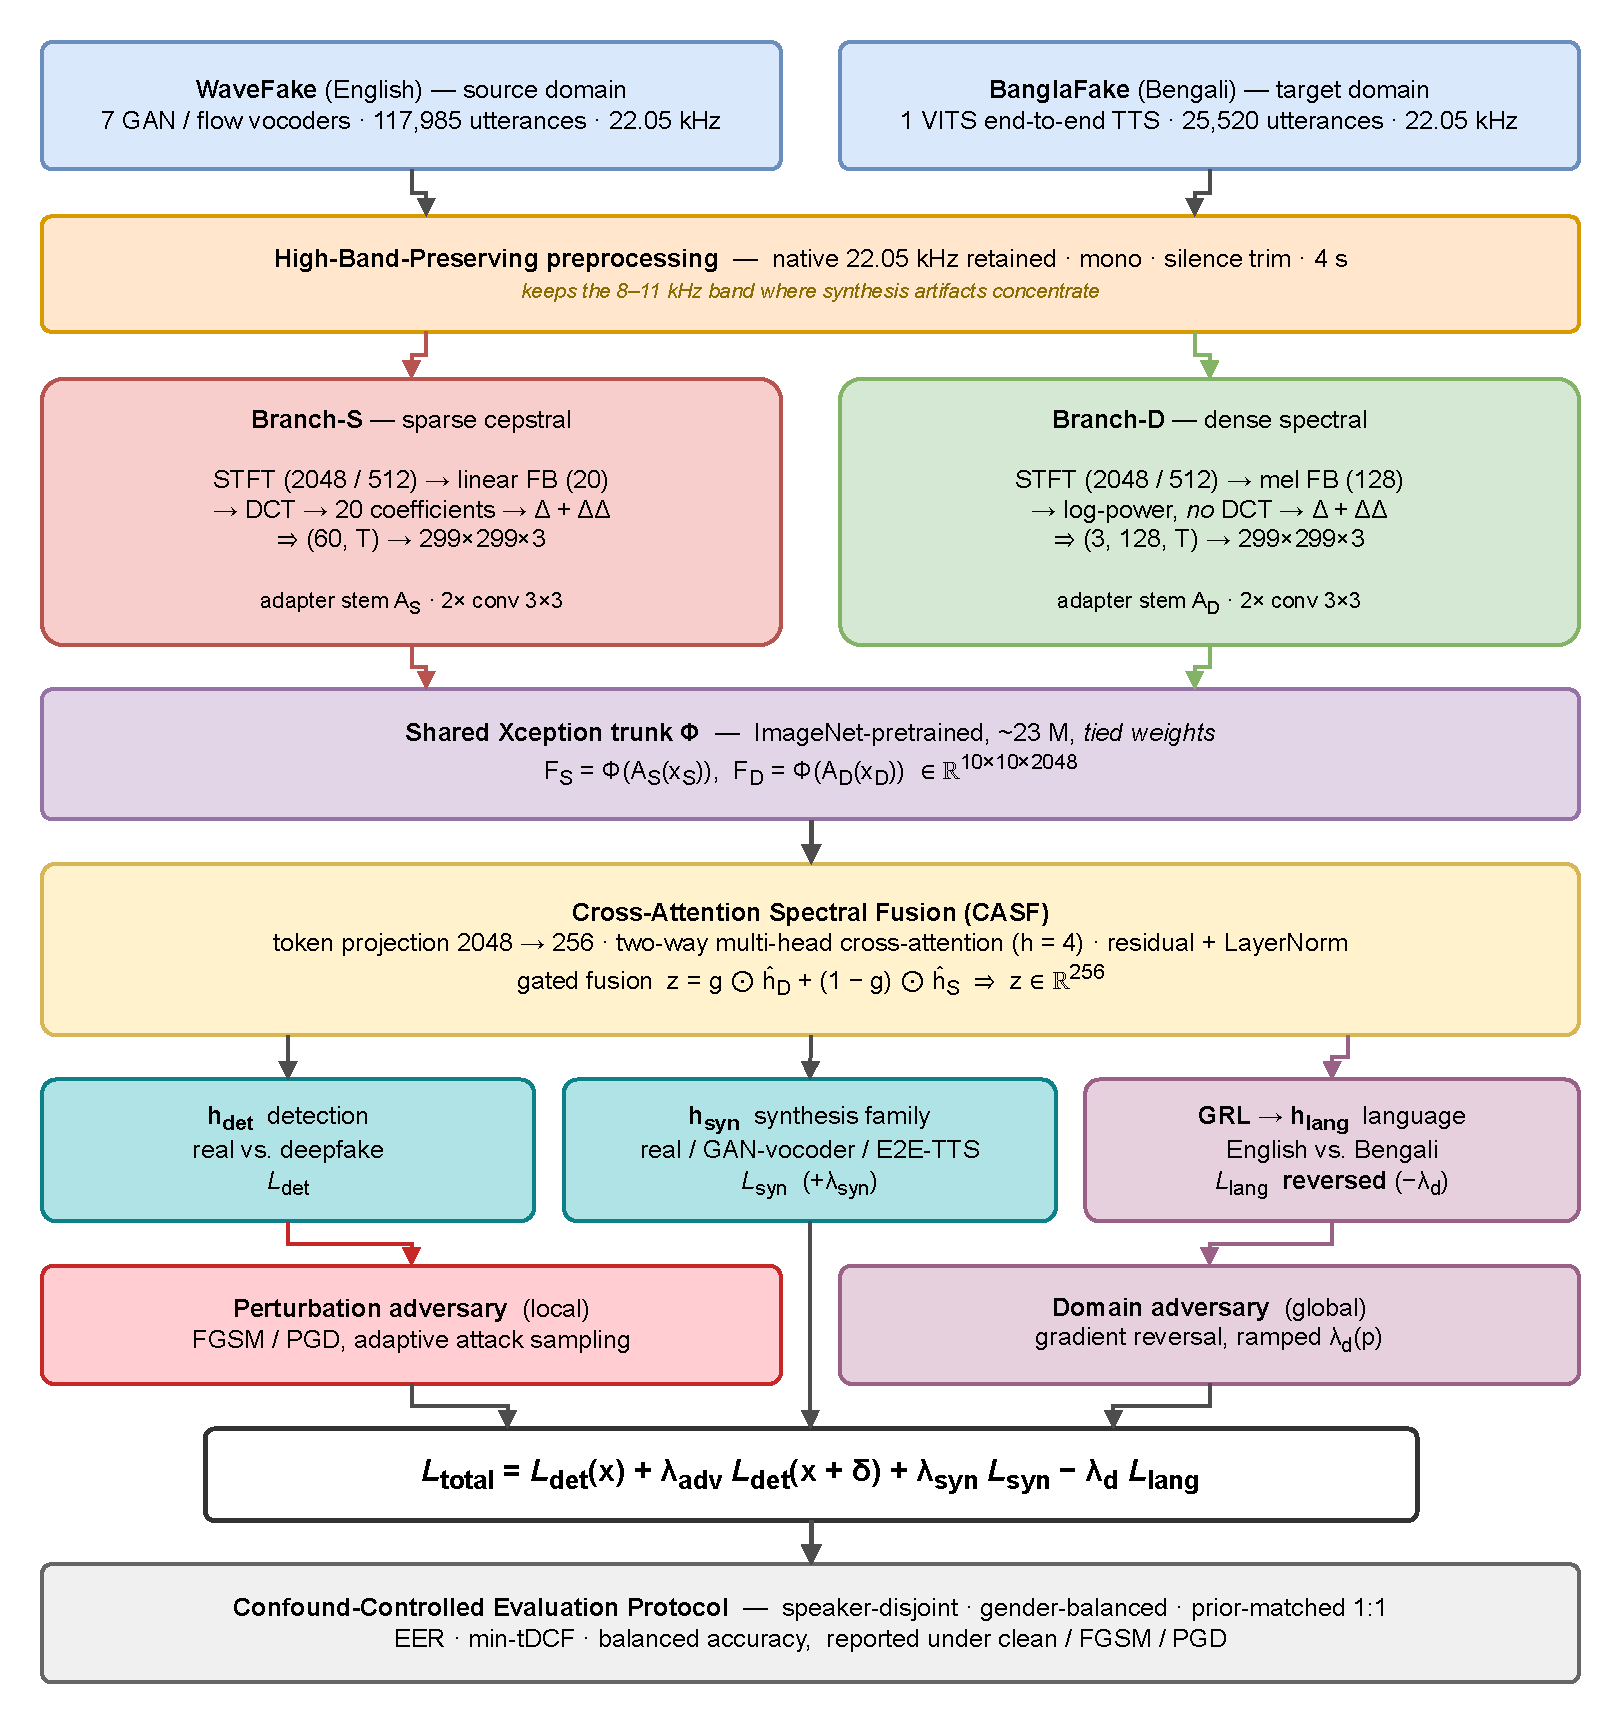
\includegraphics[width=0.86\textwidth]{fig1-methodology.drawio.pdf}
\caption{System architecture and end-to-end pipeline of DASF-Net. Both corpora
pass through identical High-Band-Preserving preprocessing, split into a sparse
cepstral and a dense spectral branch, and are encoded by one Siamese-shared
Xception trunk. Cross-Attention Spectral Fusion produces a single embedding
$z$ on which three heads act: detection, an auxiliary synthesis-family
classifier, and a gradient-reversed language discriminator. Two adversaries
--- perturbation and domain --- shape the same embedding through the combined
objective, and all reported figures follow the Confound-Controlled Evaluation
Protocol.}
\label{fig:pipeline}
\end{figure*}

\subsection{Overview of Approach}
The project is carried out in four steps. First, both corpora are normalised
to a common audio representation without discarding high-frequency content.
Second, every utterance is expressed as two complementary spectral views and
encoded by a single shared convolutional backbone. Third, the two views are
fused by a learned, attention-based gate into one embedding, on which three
prediction heads act. Fourth, that embedding is shaped by two adversaries at
once --- one local and perturbation-based, one global and domain-based ---
under a three-stage curriculum. Figure~\ref{fig:pipeline} shows the complete
system.

\subsection{Datasets}
\textbf{WaveFake (English, source domain)} \cite{frank2021wavefake} contains
117,985 utterances (13,100 real, 104,885 synthetic) built from the
single-speaker LJSpeech corpus \cite{ito2017ljspeech}, covering seven
GAN-based or GAN-adjacent flow vocoders that resynthesise a waveform from
acoustic features of real speech.

\textbf{BanglaFake (Bengali, target domain)} \cite{fahad2025banglafake}
contains 25,520 utterances: 12,260 real (10,000 from the SUST TTS Corpus,
2,260 from Common Voice across five speakers) and 13,260 synthesised by a
single VITS model trained from scratch on the SUST corpus. VITS is an
end-to-end variational/flow architecture that generates speech directly from
text, and is therefore structurally unlike every WaveFake generator. Audio is
distributed as 22{,}050~Hz WAV, 6--7~s per clip.

Because language and synthesis paradigm change together, the
English~$\leftrightarrow$~Bengali direction probes cross-lingual \emph{and}
cross-architecture generalisation at once. Table~\ref{tab:datasets} summarises
both corpora.

\begin{table}[!t]
\caption{Dataset summary after High-Band-Preserving alignment}
\label{tab:datasets}
\centering
\begin{tabular}{lcc}
\toprule
& \textbf{WaveFake} & \textbf{BanglaFake} \\
\midrule
Role                    & source        & target \\
Language                & English       & Bengali \\
Real utterances         & 13,100        & 12,260 \\
Synthetic utterances    & 104,885       & 13,260 \\
Synthesis family        & 7, GAN / flow & 1, VITS end-to-end \\
Speaker(s), synthetic   & 1 female      & 1 male \\
Speaker(s), real        & 1 female      & 7 (mixed gender) \\
Source corpus           & LJSpeech      & SUST TTS Corpus \\
Sample rate (retained)  & 22,050~Hz     & 22,050~Hz \\
\bottomrule
\end{tabular}
\end{table}

\subsection{Data Preprocessing Pipeline}
\label{sec:hbp}
Every utterance from both corpora is brought to a common representation: mono,
native 22.05~kHz \emph{retained}, silences longer than 2~s trimmed at a 40~dB
threshold, and duration normalised to 4~s by centre-cropping or reflection
padding.

Retaining the native rate is a deliberate departure from our prior pipeline.
Downsampling to 16~kHz imposes an 8~kHz Nyquist ceiling and removes the
8--11~kHz band; for a within-corpus study that loss is tolerable, but for a
cross-paradigm claim it deletes the evidence most likely to distinguish a GAN
vocoder from an end-to-end model. All filterbanks therefore run to
$f_{\max} = 11.025$~kHz. Every feature map is standardised per utterance and
squashed to $[0,1]$, so that the adversarial budget $\epsilon$ carries the
same meaning for every utterance and for both branches.

Two parallel feature pipelines share identical Short-Time Fourier Transform
parameters ($n_{\mathrm{fft}} = 2048$, hop $= 512$), so any difference between
them is attributable to the filterbank and compression stages alone:

\begin{itemize}
\item \textbf{Branch-S (sparse cepstral).} Linear-frequency filterbank
      (20 filters, 0--11.025~kHz) $\rightarrow$ Discrete Cosine Transform
      $\rightarrow$ 20 cepstral coefficients $\rightarrow$ first and second
      temporal derivatives, giving a $(60, T)$ representation.
\item \textbf{Branch-D (dense spectral).} Mel-scaled filterbank
      ($n_{\mathrm{mels}} = 128$, $f_{\max} = 11.025$~kHz) $\rightarrow$
      log-power compression, with \emph{no} DCT, so the dense
      time--frequency structure survives $\rightarrow$ first and second
      derivatives, giving a $(3, 128, T)$ tensor.
\end{itemize}

Both are resized to $299 \times 299 \times 3$, the Xception input geometry.

\subsection{System Architecture}

\begin{figure*}[!t]
\centering
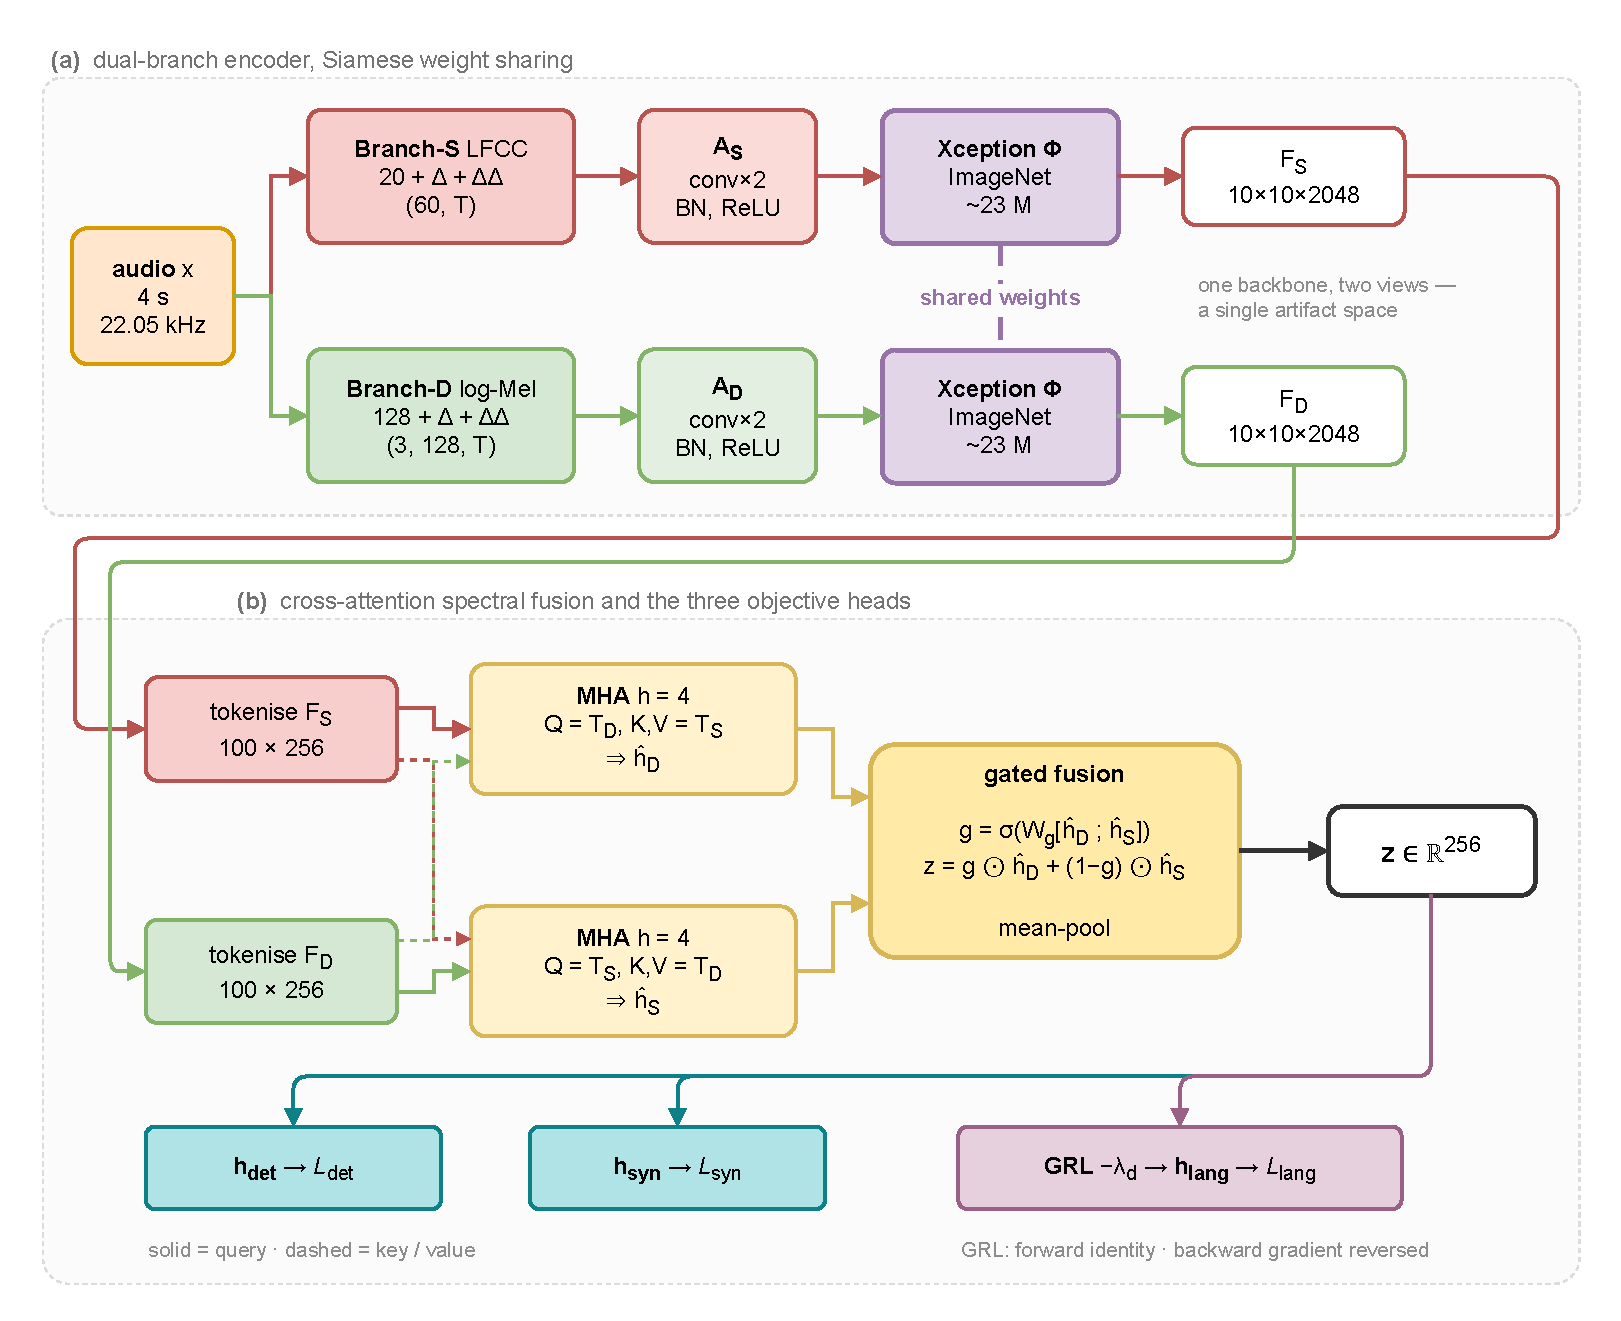
\includegraphics[width=0.98\textwidth]{fig2-dasfnet.drawio.pdf}
\caption{DASF-Net in detail. (a) The dual-branch encoder: one utterance
becomes a sparse cepstral and a dense spectral view, each passed through its
own adapter stem into a single weight-shared Xception trunk. (b) CASF
tokenises both feature maps, lets each view attend over the other, and
combines them through a learned gate into $z$; three heads then act on $z$,
the language head behind a gradient reversal layer.}
\label{fig:dasfnet}
\end{figure*}

\subsubsection{Branch adapters and a Siamese-shared trunk}
Each branch owns a small \emph{adapter stem} $A_S$, $A_D$ --- two $3\times3$
convolutions with batch normalisation and ReLU, about $0.06$~M parameters each
--- which maps branch-specific input statistics into a common range before the
shared encoder sees them. The encoder $\Phi$ is a single ImageNet-pretrained
Xception \cite{chollet2017xception} ($\approx 23$~M parameters) applied to both
branches with tied weights:
\begin{equation}
F_S = \Phi(A_S(x_S)), \qquad F_D = \Phi(A_D(x_D)),
\end{equation}
with $F_S, F_D \in \mathbb{R}^{10 \times 10 \times 2048}$.

Weight sharing is a design commitment, not an economy. Two independent
backbones would let each branch build a private feature space, and the fusion
module would then have to reconcile two unrelated geometries. One trunk forces
both views into a single artifact space at the cost of $0.12$~M extra adapter
parameters, and keeps the model comparable in size to the single-branch
baseline of \cite{ahmed2026melspec}.

\subsubsection{Cross-Attention Spectral Fusion}
Each feature map is flattened into 100 spatial tokens and linearly projected
to $d = 256$, giving $T_S, T_D \in \mathbb{R}^{100 \times 256}$. Two
multi-head cross-attention blocks \cite{vaswani2017attention} ($h = 4$) let
each view interrogate the other,
\begin{align}
\hat{h}_D &= \mathrm{LN}\!\left(T_D + \mathrm{MHA}(T_D, T_S, T_S)\right),\\
\hat{h}_S &= \mathrm{LN}\!\left(T_S + \mathrm{MHA}(T_S, T_D, T_D)\right),
\end{align}
and a learned gate mixes them elementwise before mean-pooling over tokens:
\begin{align}
g &= \sigma\!\left(W_g\,[\hat{h}_D \,;\, \hat{h}_S] + b_g\right),\\
z &= \mathrm{pool}\!\left(g \odot \hat{h}_D + (1 - g) \odot \hat{h}_S\right)
\;\in\; \mathbb{R}^{256}.
\end{align}

The gate is the point of the module. A fixed concatenation would assert that
both views always matter equally; the gate instead lets the network decide,
per utterance and per dimension, which representation carries the artifact. It
also makes the model interpretable: the distribution of $g$ over a test set is
a direct, quantitative answer to whether GAN vocoders and end-to-end TTS leave
their traces in different representations.

\subsubsection{Objective heads}
Three heads read the same $z$. The \textbf{detection head} $h_{\mathrm{det}}$
($256 \rightarrow 128 \rightarrow 2$) performs the task of record under
cross-entropy with label smoothing $0.1$. The \textbf{synthesis-family head}
$h_{\mathrm{syn}}$ ($256 \rightarrow 128 \rightarrow 3$) predicts \{real,
GAN-vocoder, end-to-end TTS\}; this supervision is deliberately coarse,
because predicting the specific generator would invite memorisation of
generator identity, which is exactly the failure that breaks cross-vocoder
transfer. The \textbf{language head} $h_{\mathrm{lang}}$ predicts English
versus Bengali but sits behind a gradient reversal layer (GRL)
\cite{ganin2016dann}, which is the identity in the forward pass and multiplies
the gradient by $-\lambda_d$ in the backward pass. The head therefore does its
best to identify the language while the shared trunk and CASF are driven to
make that identification impossible.

\subsubsection{The dual-adversarial objective}
Writing $\delta$ for an adversarial perturbation of the input features, the
complete training objective is
\begin{equation}
\label{eq:total}
\Loss_{\mathrm{total}} =
\Loss_{\mathrm{det}}(x)
+ \lambda_{\mathrm{adv}} \Loss_{\mathrm{det}}(x + \delta)
+ \lambda_{\mathrm{syn}} \Loss_{\mathrm{syn}}
- \lambda_{d} \Loss_{\mathrm{lang}} ,
\end{equation}
where the negative sign is realised by the GRL rather than by ascending the
loss directly. The perturbation adversary is \emph{local}: it searches a small
neighbourhood of each input for a direction that flips the decision. The
domain adversary is \emph{global}: it searches the embedding for any direction
that reveals the corpus. Our hypothesis is that they are complementary, and
the ablation of Section~\ref{sec:testing} is designed to test that hypothesis
rather than assume it.

\subsection{Training Pipeline}

\begin{figure*}[!t]
\centering
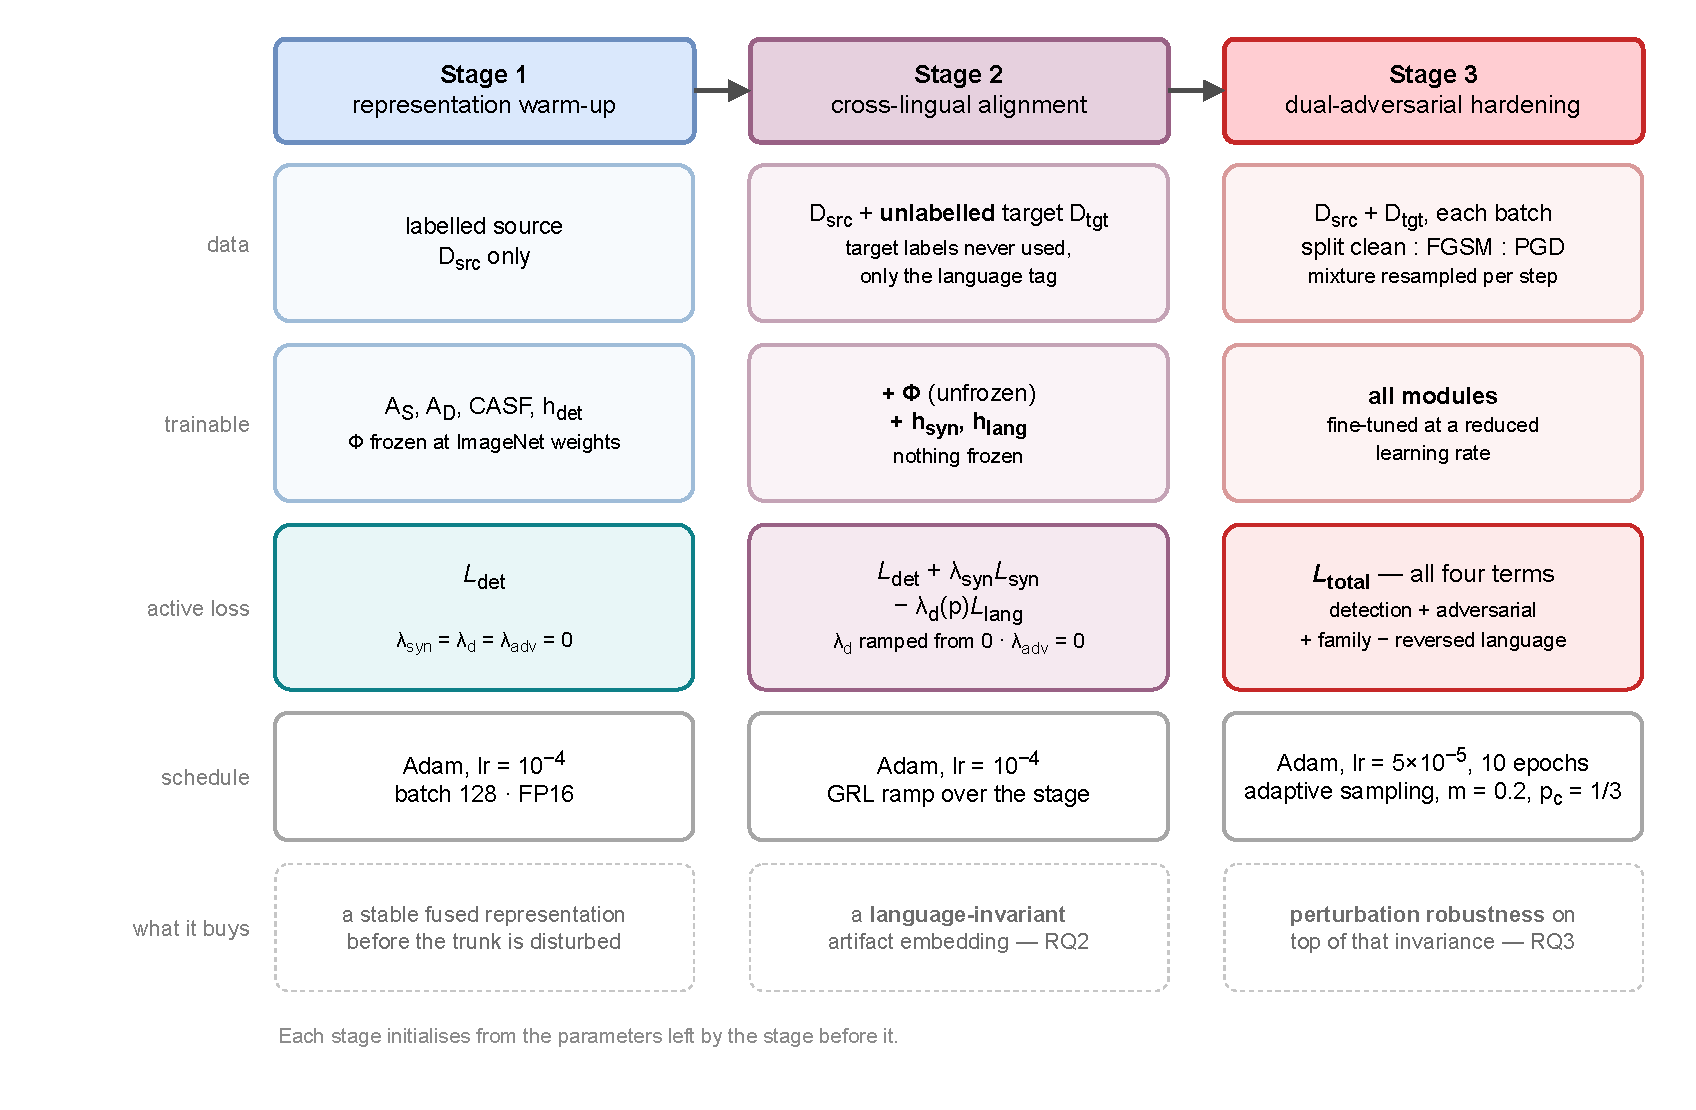
\includegraphics[width=0.98\textwidth]{fig3-training.drawio.pdf}
\caption{The three-stage training curriculum. Each stage adds one source of
difficulty and inherits the weights of the stage before it.}
\label{fig:training}
\end{figure*}

Training equation~(\ref{eq:total}) from random initialisation is unstable in
practice: a gradient-reversed discriminator applied to an untrained encoder
produces a large, uninformative reversed gradient, and adversarial examples
generated against an untrained decision boundary are meaningless. Difficulty
is therefore introduced in three stages (Fig.~\ref{fig:training}), each
initialised from the previous.

\textbf{Stage 1 --- representation warm-up.} $\Phi$ is frozen at its ImageNet
weights; only $A_S$, $A_D$, CASF and $h_{\mathrm{det}}$ train, on labelled
source data, under $\Loss_{\mathrm{det}}$ alone. Adam, $lr = 10^{-4}$,
effective batch 128 (micro-batch 16, accumulation 8), mixed precision.

\textbf{Stage 2 --- cross-lingual alignment.} $\Phi$ unfreezes;
$h_{\mathrm{syn}}$ and $h_{\mathrm{lang}}$ are attached. Batches mix labelled
source audio with \emph{unlabelled} target audio: target labels are never
used, only the language tag, which keeps the setting honestly unsupervised
with respect to the target domain. Following \cite{ganin2016dann} the reversal
coefficient is ramped rather than fixed,
\begin{equation}
\lambda_d(p) = \lambda_{\max}\left(\frac{2}{1 + e^{-10p}} - 1\right),
\end{equation}
with $p \in [0,1]$ the fraction of the stage completed.

\textbf{Stage 3 --- dual-adversarial hardening.} All modules fine-tune at
$lr = 5 \times 10^{-5}$ for 10 epochs with adversarial examples, the language
adversary still active. Rather than fixing the ratio of FGSM to PGD batches,
the attack for each minibatch is sampled in proportion to a momentum-smoothed
estimate of how successful each attack has recently been,
\begin{equation}
s_a \leftarrow (1 - m)\, s_a + m\, \hat{s}_a, \qquad m = 0.2,
\end{equation}
while a fixed fraction $p_c = 1/3$ of every minibatch stays clean to preserve
baseline accuracy.

\subsection{Testing Pipeline and Threat Model}
\label{sec:threat}
Two white-box attacks are evaluated in the normalised feature domain, where
inputs lie in $[0,1]$. FGSM \cite{goodfellow2015fgsm} takes a single step,
$\delta = \epsilon \cdot \mathrm{sign}(\nabla_x \Loss_{\mathrm{det}})$, and
PGD \cite{madry2018pgd} iterates $K = 10$ steps with step size
$\alpha = \epsilon / 4$, projecting onto the $\ell_\infty$ ball of radius
$\epsilon$ after each step. Critically, \emph{both attacks are swept over the
same $\epsilon$ grid}, $\epsilon \in \{0.001,\, 0.005,\, 0.010\}$. Prior work,
including our own, reports FGSM and PGD at $\epsilon$ values two orders of
magnitude apart, which makes the resulting robustness figures non-comparable
between the two attacks.

\subsection{Tools and Resources}
Table~\ref{tab:tools} lists the software and hardware used. All software is
open source and both datasets are publicly available at no cost.

\begin{table}[!t]
\caption{Tools, resources and technologies}
\label{tab:tools}
\centering
\renewcommand{\arraystretch}{1.15}
\begin{tabular}{@{}ll@{}}
\toprule
\textbf{Component} & \textbf{Choice} \\
\midrule
Language / framework  & Python 3, PyTorch \\
Pretrained backbones  & \texttt{timm} (ImageNet Xception) \\
Audio processing      & \texttt{librosa}, \texttt{soundfile}, \texttt{scipy} \\
Metrics               & \texttt{scikit-learn} (ROC / EER) \\
Data handling         & \texttt{numpy}, \texttt{pandas} \\
Attacks               & implemented directly in PyTorch autograd \\
Source dataset        & WaveFake (public) \\
Target dataset        & BanglaFake (HuggingFace, public) \\
Diagrams              & draw.io \\
Typesetting           & \LaTeX{} (IEEEtran) \\
Compute               & NVIDIA RTX 5060 Ti, 8~GB (local) \\
\bottomrule
\end{tabular}
\end{table}

The 8~GB VRAM budget is a binding design constraint rather than an incidental
detail. Because the shared trunk is evaluated twice per utterance, one sample
occupies roughly double the activation memory of a single-branch Xception at
$299 \times 299$ input, and a nominal batch of 128 does not fit. All training
therefore uses a \textbf{micro-batch of 16 with gradient accumulation over 8
steps}, giving an effective batch of 128 and preserving the optimisation
behaviour assumed by the learning rates above, at the cost of additional
wall-clock time. Mixed precision (FP16) is used throughout, and adversarial
examples are generated with the model parameters detached so that only input
gradients are retained.

% =============================================================================
\section{Testing Methodology}
\label{sec:testing}
% ------------------------------------------------- guideline 7

\subsection{How Success Will Be Measured}
Success is defined against the four objectives of Section~I, and is measured
by the following criteria.

\subsubsection{Evaluation metrics}
The headline metric is \textbf{Equal Error Rate (EER)}, the operating point on
the ROC curve where the false positive rate equals the false negative rate.
EER is threshold-free, which matters here because the source corpus has a
roughly 8:1 synthetic-to-real prior and the target corpus a roughly 1:1 prior;
a threshold calibrated on one is miscalibrated on the other. \textbf{Balanced
accuracy} is reported alongside it. Raw accuracy is never reported for a
transfer condition without its matching prior.

The project's evaluation plan also names min-tDCF, a standard anti-spoofing
metric. It should be recorded explicitly that min-tDCF is defined over a
\emph{tandem} system --- a countermeasure plus an automatic speaker
verification subsystem --- and that neither WaveFake nor BanglaFake ships ASV
scores. It is therefore not computable from this data without adding an ASV
subsystem, and is not reported.

\subsubsection{Benchmarks}
Three published reference points are used: the ResNet18 fine-tuned baseline on
BanglaFake at 79.17\% accuracy / 0.2435 EER \cite{samu2025zeroshot}; the
single-branch Xception with log-Mel at 0.034 average EER on WaveFake
\cite{ahmed2026melspec}; and the GMM+LFCC classical baseline at 0.058 EER
\cite{frank2021wavefake}.

\subsubsection{Confound-Controlled Evaluation Protocol}
Every reported figure is subject to four constraints, which follow from the
confounds identified in Section~III:

\begin{enumerate}
\item \textbf{Speaker-disjoint splits.} No speaker appears in both training
      and test partitions, so a model cannot succeed by speaker recognition.
\item \textbf{Gender-balanced Bengali evaluation.} Because BanglaFake pairs
      one male synthetic speaker against mixed-gender real speech, the primary
      Bengali test set is restricted to male real speech, and the
      mixed-gender result is reported separately as a diagnostic. A large gap
      between the two is itself evidence of gender shortcutting.
\item \textbf{Prior-matched test sets.} Both test sets are resampled to
      $1{:}1$ real-to-synthetic.
\item \textbf{Threshold-free primary metric}, as above.
\end{enumerate}

\subsubsection{Experiments}
Five experiments are planned, summarised in Table~\ref{tab:experiments}.

\begin{table}[!t]
\caption{Planned experiments and the objective each addresses}
\label{tab:experiments}
\centering
\renewcommand{\arraystretch}{1.2}
\begin{tabularx}{\columnwidth}{@{}l >{\raggedright\arraybackslash}X c@{}}
\toprule
\textbf{ID} & \textbf{Experiment} & \textbf{Obj.} \\
\midrule
E1 & In-language baselines: Branch-S only, Branch-D only, and full CASF
     fusion, per corpus & 2 \\
E2 & Zero-shot transfer in both directions, with and without the language
     adversary; per-vocoder breakdown; $\leq$10\% few-shot variant & 3 \\
E3 & Clean, FGSM and PGD EER per $\epsilon$, in-domain versus transferred
     robustness & 4 \\
E4 & \textbf{Ablation}: remove CASF, shared trunk, $h_{\mathrm{syn}}$, GRL,
     adversarial stage, or HBP, one at a time & 1--4 \\
E5 & Gate analysis: distribution of $g$ per synthesis family & 1 \\
\bottomrule
\end{tabularx}
\end{table}

E4 is the experiment that converts an observed improvement into an attributed
one. Without it, any gain remains unexplained; with it, the contribution of
each component can be isolated. All experiments are run with three random
seeds and reported as mean and standard deviation; single-seed results are not
reported.

\subsubsection{Achievement of objectives}
Objective~1 is met when the implementation passes its correctness tests
(tensor shapes, gradient-reversal sign flip, attack budget compliance).
Objectives~2--4 are met when E1, E2 and E3 respectively produce
seed-averaged EER figures under CCEP, whatever those figures turn out to be.
A negative result --- for instance, that the language adversary does not
improve transfer --- satisfies the objective provided it is measured under a
protocol that could have detected an improvement.

\subsection{Monitoring and Reporting}
Progress is monitored through weekly supervisor meetings, a shared Git
repository with all code and experiment configurations committed, and
per-epoch training logs recording each loss term separately
($\Loss_{\mathrm{det}}$, $\Loss_{\mathrm{syn}}$, $\Loss_{\mathrm{lang}}$) plus
the running attack-success estimates. Recording the loss terms separately is
what makes the GRL diagnosable: a language loss that collapses toward chance
indicates the adversary is working, while one that collapses toward zero
indicates it has overwhelmed the encoder.

\subsection{Current Status}
No experiments have yet been executed. The architecture, the training
algorithms, the threat model and the evaluation protocol are complete and the
reference implementation is written, but it has not been trained, and this
report therefore contains no results, no accuracy figures and no trained
model. Reporting this plainly is preferred to presenting an untested design as
a validated one.

% =============================================================================
\section{Project Timeline}
% ------------------------------------------------- guideline 8
Table~\ref{tab:timeline} lists the phases and their status. Note that
Phases~4 and~5 fall after the report deadline of 6 September 2026: the design
and implementation were completed within the reporting period, but the
training runs were not.

\begin{table}[!t]
\caption{Project timeline and milestones}
\label{tab:timeline}
\centering
\renewcommand{\arraystretch}{1.2}
\begin{tabularx}{\columnwidth}{@{}l >{\raggedright\arraybackslash}X l@{}}
\toprule
\textbf{Phase} & \textbf{Activity} & \textbf{Status} \\
\midrule
1 & Literature review; dataset acquisition and manifest construction
    \newline \emph{May--Jun 2026} & Complete \\
2 & Architecture design; algorithm specification; diagrams; reference
    implementation \newline \emph{Jun--Aug 2026} & Complete \\
3 & Report preparation and submission
    \newline \emph{Aug--6 Sep 2026} & Complete \\
4 & Environment setup; training runs E1--E3
    \newline \emph{from 6 Sep 2026} & In progress \\
5 & Ablation E4 and gate analysis E5; results write-up
    \newline \emph{after Phase 4} & Pending \\
\bottomrule
\end{tabularx}
\end{table}

The critical-path risk is Phase~4: the dependency install and the first full
training run must both succeed before Phase~5 can begin. Mitigation is
described in Section~IX.

% =============================================================================
\section{Budget}
% ------------------------------------------------- guideline 9
Training runs on a locally owned NVIDIA RTX 5060 Ti (8~GB), so the project
incurs almost no direct monetary cost; the real cost is time and electricity.
Table~\ref{tab:budget} gives the estimate. Compute demand is driven by two
architectural decisions: the shared trunk runs twice per utterance, roughly
doubling forward and backward cost relative to a single-branch model, and
Stage~3 adversarial training with PGD at $K = 10$ multiplies the cost of every
attacked minibatch. The estimate assumes on the order of 200 GPU-hours across
all experiments and three seeds. The electricity and currency figures are
order-of-magnitude estimates, assuming 1~USD $\approx$ 120~BDT, 8~BDT/kWh,
and a sustained draw of about 0.2~kW.

\begin{table}[!t]
\caption{Estimated project budget}
\label{tab:budget}
\centering
\renewcommand{\arraystretch}{1.2}
\begin{tabularx}{\columnwidth}{@{}>{\raggedright\arraybackslash}X r r@{}}
\toprule
\textbf{Item} & \textbf{USD} & \textbf{BDT} \\
\midrule
Personnel (2 students, academic credit)        & 0   & 0 \\
GPU hardware (RTX 5060 Ti, already owned)      & 0   & 0 \\
Electricity, $\approx$200 GPU-h @ 0.2 kW       & 3   & 320 \\
Storage, $\approx$150 GB local disk            & 0   & 0 \\
Software and tools (all open source)           & 0   & 0 \\
Datasets (both publicly released)              & 0   & 0 \\
\midrule
\textbf{Total, direct cost}                    & \textbf{3} & \textbf{320} \\
\midrule
\emph{Contingency: cloud fallback if local}    &     & \\
\emph{training proves infeasible ($\approx$200 h)} & \emph{300} & \emph{36,000} \\
\bottomrule
\end{tabularx}
\end{table}

The direct monetary cost is therefore negligible; the binding resource is the
8~GB VRAM ceiling and the wall-clock time that the resulting micro-batching
implies. The contingency line is not part of the planned spend --- it is the
cost that would be incurred only if the local card cannot complete the runs
within the available time, and it is listed so that the fallback is costed
rather than assumed free.

% =============================================================================
\section{Team Members and Roles}
% ------------------------------------------------- guideline 10
The two student members contributed equally, taking ten report sections each
as itemised in the Individual Contribution Table.

\begin{itemize}
\item \textbf{Iftikhar Ahmed} (2121019642) --- model and method. Architecture
      design (CASF, the dual-adversarial objective, the three-stage
      curriculum), reference implementation, adversarial threat model,
      testing methodology, risk analysis, system diagrams, and \LaTeX{}
      preparation of the report.
\item \textbf{Meherun Nessa Mithila} (2221649042) --- data and evaluation.
      Literature review and the five paper reviews, dataset acquisition and
      manifest construction, preprocessing pipeline, evaluation protocol,
      timeline and budget, and language editing.
\item \textbf{Mohammad Abdul Qayum}, Assistant Professor, ECE Department ---
      course faculty and supervisor. Scope definition, methodological review,
      and approval of the evaluation protocol.
\end{itemize}

A per-section breakdown of contributions is given in the Individual
Contribution Table on the second page of this report.

% =============================================================================
\section{Risks and Mitigation Strategies}
% ------------------------------------------------- guideline 11

\textbf{Risk 1 --- Gradient reversal fails to converge.} The GRL is a
known-unstable component; an overly aggressive reversal coefficient can
destroy the encoder's discriminative capacity.
\emph{Mitigation:} the GRL is introduced only in Stage~2, never at
initialisation, and $\lambda_d$ is ramped from zero by the standard DANN
schedule. The language loss is logged separately so divergence is visible
immediately. If it still fails, the fallback is a non-adversarial alignment
objective such as maximum mean discrepancy, and the failure is reported as a
negative result rather than concealed.

\textbf{Risk 2 --- The gender confound inflates Bengali results.} BanglaFake's
synthetic side is one male speaker against mixed-gender real speech, so a
model can score highly by classifying gender.
\emph{Mitigation:} CCEP restricts the primary Bengali test set to male real
speech and reports the mixed-gender figure separately as a diagnostic; a
large gap between them is treated as evidence of shortcutting rather than
success.

\textbf{Risk 3 --- Compute and memory ceiling.} Training runs on a single
8~GB RTX 5060 Ti. The two-branch encoder roughly doubles both activation
memory and training cost, and PGD at $K = 10$ multiplies the cost further; the
full 117,985-utterance WaveFake corpus at three seeds is unlikely to fit in
the available wall-clock time. This is the most probable cause of the project
failing to produce results.
\emph{Mitigation:} the micro-batch of 16 with gradient accumulation over 8
steps keeps the effective batch at 128 within the VRAM ceiling. WaveFake is
subsampled to a prior-matched subset, reducing 117,985 utterances to roughly
26,000 without changing the design --- for this hardware, subsampling is a
necessity rather than an option. PGD steps are reduced to $K = 5$ for
ablation runs, with the full $K = 10$ budget reserved for the headline E3
numbers, and gradient checkpointing on the shared trunk is held in reserve if
memory still binds.

\textbf{Risk 4 --- Only one Bengali generator exists.} With a single VITS
system, cross-vocoder generalisation within Bengali cannot be tested.
\emph{Mitigation:} claims are scoped explicitly to cross-\emph{paradigm}
transfer, and the limitation is stated in the report rather than left for a
reviewer to find. Adding a Bengali FastSpeech2 or Tacotron2 system is
identified as the next step.

\textbf{Risk 5 --- Schedule slip leaves the project without results.} Phase~3
is on the critical path and depends on a successful environment setup.
\emph{Mitigation:} experiments are prioritised so that E1 and E2 --- which
answer Objectives~2 and~3 --- run first; E4 and E5 are valuable but
deferrable. A smoke test that exercises every code path on random tensors,
without any dataset or pretrained download, allows the implementation to be
validated before compute is committed.

\textbf{Risk 6 --- Environment and dependency failure.} The project depends on
PyTorch, timm and librosa, none of which is currently installed on the
development machine, and the pretrained Xception weights require a download.
\emph{Mitigation:} the implementation accepts an injected backbone, so it can
be validated with a lightweight stand-in trunk before the real dependency
stack is installed.

% =============================================================================
\section{Conclusion and Limitations}
% ------------------------------------------------- guideline 12
This project proposes DASF-Net, an architecture that treats the two standing
weaknesses of audio deepfake detectors --- brittleness across languages and
brittleness under perturbation --- as instances of the same problem, and
attacks both with adversaries acting on one shared embedding. It contributes a
dual-branch spectral front-end over a Siamese-shared Xception trunk, a gated
cross-attention fusion module that learns per utterance which spectral view
carries the artifact, a combined objective in which a gradient-reversed
language discriminator and adaptive FGSM/PGD training shape the same
representation, a three-stage curriculum that makes this trainable, a
corrected and unit-consistent adversarial threat model, and an evaluation
protocol that neutralises the speaker, gender and prior imbalances which
otherwise make Bengali detection results unreadable.

The work is positioned to be publishable because it addresses two problems
that the most recent Bengali detection benchmark \cite{samu2025zeroshot}
explicitly named as open, and because it does so with a mechanism rather than
with more data or a larger model. If the central hypothesis holds, the result
is a detector whose features describe what a synthesiser did rather than which
corpus it was trained on --- a property that generalises beyond Bengali to any
low-resource language with unlabelled speech available.

\subsection{Limitations}
Several limitations bound what this project can conclude, and are stated in
advance rather than discovered later.

\begin{itemize}
\item \textbf{No results yet.} The experiments of Section~V have not been
      executed. Every claim in this report is a design claim, not an empirical
      one.
\item \textbf{One Bengali generator.} BanglaFake contains a single VITS
      system, so the design tests cross-paradigm generalisation but cannot
      test cross-vocoder generalisation within Bengali the way WaveFake's
      seven-generator protocol does for English. No such claim is made.
\item \textbf{Confounds mitigated, not eliminated.} CCEP controls speaker,
      gender and prior, but each control shrinks the usable Bengali evaluation
      set, trading statistical power for validity.
\item \textbf{White-box attacks only.} FGSM and PGD assume full gradient
      access. Black-box, transfer, perceptual and physical-channel attacks are
      outside this design.
\item \textbf{Two languages.} Bengali and English differ in phoneme inventory,
      prosody and recording conditions simultaneously, so invariance
      demonstrated over one pair is evidence, not proof, of invariance in
      general.
\item \textbf{Computational cost.} Stage~3 roughly doubles training time on
      top of the already doubled forward cost of the two-branch encoder.
\end{itemize}

% =============================================================================
\begin{thebibliography}{00}

\bibitem{kong2020hifigan}
J.~Kong, J.~Kim, and J.~Bae, ``HiFi-GAN: Generative adversarial networks for
efficient and high fidelity speech synthesis,'' in \emph{Advances in Neural
Information Processing Systems (NeurIPS)}, vol.~33, 2020, pp.~17022--17033.

\bibitem{kumar2019melgan}
K.~Kumar, R.~Kumar, T.~de~Boissiere, L.~Gestin, W.~Z.~Teoh, J.~Sotelo,
A.~de~Br\'{e}bisson, Y.~Bengio, and A.~Courville, ``MelGAN: Generative
adversarial networks for conditional waveform synthesis,'' in \emph{Advances
in Neural Information Processing Systems (NeurIPS)}, vol.~32, 2019,
pp.~14910--14921.

\bibitem{prenger2019waveglow}
R.~J.~Prenger, R.~Valle, and B.~Catanzaro, ``WaveGlow: A flow-based generative
network for speech synthesis,'' in \emph{Proc.\ ICASSP}, 2019, pp.~3617--3621.

\bibitem{yamamoto2020pwg}
R.~Yamamoto, E.~Song, and J.-M.~Kim, ``Parallel WaveGAN: A fast waveform
generation model based on generative adversarial networks with
multi-resolution spectrogram,'' in \emph{Proc.\ ICASSP}, 2020, pp.~6199--6203.

\bibitem{kim2021vits}
J.~Kim, J.~Kong, and J.~Son, ``Conditional variational autoencoder with
adversarial learning for end-to-end text-to-speech,'' in \emph{Proc.\
International Conference on Machine Learning (ICML)}, 2021, pp.~5530--5540.

\bibitem{todisco2019asvspoof}
M.~Todisco, X.~Wang, V.~Vestman, M.~Sahidullah, H.~Delgado, A.~Nautsch,
J.~Yamagishi, N.~Evans, T.~H.~Kinnunen, and K.~A.~Lee, ``ASVspoof 2019: Future
horizons in spoofed and fake audio detection,'' in \emph{Proc.\ Interspeech},
2019, pp.~1008--1012.

\bibitem{frank2021wavefake}
J.~Frank and L.~Sch\"{o}nherr, ``WaveFake: A data set to facilitate audio
deepfake detection,'' in \emph{35th Conference on Neural Information
Processing Systems (NeurIPS) Datasets and Benchmarks Track}, 2021.

\bibitem{fahad2025banglafake}
I.~A.~Fahad, K.~Asif, and S.~Sikder, ``BanglaFake: Constructing and evaluating
a specialized Bengali deepfake audio dataset,'' \emph{arXiv preprint
arXiv:2505.10885}, 2025.

\bibitem{samu2025zeroshot}
M.~S.~S.~Samu, M.~R.~Islam, M.~Z.~Hossain, M.~K.~Bhuiyan, and F.~U.~Zaman,
``Zero-shot to zero-lies: Detecting Bengali deepfake audio through transfer
learning,'' in \emph{2025 28th International Conference on Computer and
Information Technology (ICCIT)}, 2025.

\bibitem{ahmed2026melspec}
I.~Ahmed, M.~I.~Arian, and N.~J.~Lisa, ``Mel-Spectrogram representations for
CNN based adversarial defense for audio deepfake detection,''
in \emph{Proc.\ 2026 11th International Conference on Machine Learning
Technologies (ICMLT)}, Berlin, Germany, 2026.

\bibitem{chollet2017xception}
F.~Chollet, ``Xception: Deep learning with depthwise separable convolutions,''
in \emph{Proc.\ IEEE Conf.\ on Computer Vision and Pattern Recognition
(CVPR)}, 2017, pp.~1800--1807.

\bibitem{ganin2016dann}
Y.~Ganin, E.~Ustinova, H.~Ajakan, P.~Germain, H.~Larochelle, F.~Laviolette,
M.~Marchand, and V.~Lempitsky, ``Domain-adversarial training of neural
networks,'' \emph{Journal of Machine Learning Research}, vol.~17, no.~59,
pp.~1--35, 2016.

\bibitem{vaswani2017attention}
A.~Vaswani, N.~Shazeer, N.~Parmar, J.~Uszkoreit, L.~Jones, A.~N.~Gomez,
{\L}.~Kaiser, and I.~Polosukhin, ``Attention is all you need,'' in
\emph{Advances in Neural Information Processing Systems (NeurIPS)}, vol.~30,
2017, pp.~5998--6008.

\bibitem{goodfellow2015fgsm}
I.~J.~Goodfellow, J.~Shlens, and C.~Szegedy, ``Explaining and harnessing
adversarial examples,'' in \emph{Proc.\ ICLR}, 2015.

\bibitem{madry2018pgd}
A.~Madry, A.~Makelov, L.~Schmidt, D.~Tsipras, and A.~Vladu, ``Towards deep
learning models resistant to adversarial attacks,'' in \emph{Proc.\ ICLR},
2018.

\bibitem{kawa2023lcnn}
P.~Kawa, M.~Plata, and P.~Syga, ``Defense against adversarial attacks on audio
deepfake detection,'' in \emph{Proc.\ Interspeech}, 2023, pp.~5276--5280.

\bibitem{ito2017ljspeech}
K.~Ito and L.~Johnson, ``The LJ speech dataset,''
\url{https://keithito.com/LJ-Speech-Dataset/}, 2017.

\bibitem{ahmad2021sust}
A.~Ahmad, M.~Selim, M.~Iqbal, and M.~Rahman, ``SUST TTS corpus: A
phonetically balanced corpus for Bangla text-to-speech synthesis,''
\emph{Acoustical Science and Technology}, vol.~42, no.~6, pp.~326--332, 2021.

\bibitem{ardila2020commonvoice}
R.~Ardila, M.~Branson, K.~Davis, M.~Henretty, M.~Kohler, J.~Meyer, R.~Morais,
L.~Saunders, F.~M.~Tyers, and G.~Weber, ``Common Voice: A
massively-multilingual speech corpus,'' in \emph{Proc.\ 12th Conference on
Language Resources and Evaluation (LREC)}, 2020, pp.~4211--4215.

\end{thebibliography}

\end{document}
